\batchmode
\documentclass[a4paper]{book}
\usepackage{makeidx}
\usepackage{graphicx}
\usepackage{multicol}
\usepackage{float}
\usepackage{listings}
\usepackage{color}
\usepackage{ifthen}
\usepackage[table]{xcolor}
\usepackage{textcomp}
\usepackage{alltt}
\usepackage[utf8]{inputenc}
\usepackage{mathptmx}
\usepackage[scaled=.90]{helvet}
\usepackage{courier}
\usepackage{sectsty}
\usepackage[titles]{tocloft}
\usepackage{doxygen}
\lstset{language=C++,inputencoding=utf8,basicstyle=\footnotesize,breaklines=true,breakatwhitespace=true,tabsize=8,numbers=left }
\makeindex
\setcounter{tocdepth}{3}
\renewcommand{\footrulewidth}{0.4pt}
\renewcommand{\familydefault}{\sfdefault}
\begin{document}
\begin{titlepage}
\vspace*{7cm}
\begin{center}
{\Large mixed\_\-real\_\-c }\\
\vspace*{1cm}
{\large Generated by Doxygen 1.7.4}\\
\vspace*{0.5cm}
{\small Wed May 15 2013 14:02:35}\\
\end{center}
\end{titlepage}
\clearemptydoublepage
\pagenumbering{roman}
\tableofcontents
\clearemptydoublepage
\pagenumbering{arabic}
\chapter{Main Page}
\label{index}

{\bfseries rosconsole} is a package for console output and logging. It provides a macro-\/based interface which allows both printf-\/ and stream-\/style output. It also wraps \doxyref{log4cxx}{p.}{namespacelog4cxx} ({\tt http://logging.apache.org/log4cxx/index.html}), which supports hierarchical loggers, verbosity levels and configuration-\/files. 
\chapter{Class Index}
\section{Class List}
Here are the classes, structs, unions and interfaces with brief descriptions:\begin{DoxyCompactList}
\item\contentsline{section}{{\bf AdvancedFilter} }{\pageref{structAdvancedFilter}}{}
\item\contentsline{section}{{\bf BasicFilter} }{\pageref{structBasicFilter}}{}
\item\contentsline{section}{{\bf ChangeFilter} }{\pageref{structChangeFilter}}{}
\item\contentsline{section}{{\bf ros::console::FileToken} }{\pageref{structros_1_1console_1_1FileToken}}{}
\item\contentsline{section}{{\bf ros::console::FilterBase} (Base-\/class for filters. Filters allow full user-\/defined control over whether or not a message should print. The ROS\_\-X\_\-FILTER... macros provide the filtering functionality )}{\pageref{classros_1_1console_1_1FilterBase}}{}
\item\contentsline{section}{{\bf ros::console::FilterParams} (Parameter structure passed to \doxyref{FilterBase::isEnabled}{p.}{classros_1_1console_1_1FilterBase_ac4a1c9d0ba5672f7cdd0f3e72014fb27}(...);. Includes both input and output parameters )}{\pageref{structros_1_1console_1_1FilterParams}}{}
\item\contentsline{section}{{\bf ros::console::FixedMapToken} }{\pageref{structros_1_1console_1_1FixedMapToken}}{}
\item\contentsline{section}{{\bf ros::console::FixedToken} }{\pageref{structros_1_1console_1_1FixedToken}}{}
\item\contentsline{section}{{\bf ros::console::Formatter} }{\pageref{structros_1_1console_1_1Formatter}}{}
\item\contentsline{section}{{\bf ros::console::FunctionToken} }{\pageref{structros_1_1console_1_1FunctionToken}}{}
\item\contentsline{section}{{\bf TestAppender::Info} }{\pageref{structTestAppender_1_1Info}}{}
\item\contentsline{section}{{\bf ros::console::LineToken} }{\pageref{structros_1_1console_1_1LineToken}}{}
\item\contentsline{section}{{\bf ros::console::LoggerToken} }{\pageref{structros_1_1console_1_1LoggerToken}}{}
\item\contentsline{section}{{\bf ros::console::LogLocation} (Internal )}{\pageref{structros_1_1console_1_1LogLocation}}{}
\item\contentsline{section}{{\bf ros::console::MessageToken} }{\pageref{structros_1_1console_1_1MessageToken}}{}
\item\contentsline{section}{{\bf ros::console::PlaceHolderToken} }{\pageref{structros_1_1console_1_1PlaceHolderToken}}{}
\item\contentsline{section}{{\bf ros::console::ROSConsoleStdioAppender} }{\pageref{classros_1_1console_1_1ROSConsoleStdioAppender}}{}
\item\contentsline{section}{{\bf ros::console::SeverityToken} }{\pageref{structros_1_1console_1_1SeverityToken}}{}
\item\contentsline{section}{{\bf ros::console::StaticInit} }{\pageref{classros_1_1console_1_1StaticInit}}{}
\item\contentsline{section}{{\bf TestAppender} }{\pageref{classTestAppender}}{}
\item\contentsline{section}{{\bf TestAppenderWithThrow} }{\pageref{classTestAppenderWithThrow}}{}
\item\contentsline{section}{{\bf ros::console::ThreadToken} }{\pageref{structros_1_1console_1_1ThreadToken}}{}
\item\contentsline{section}{{\bf ros::console::TimeToken} }{\pageref{structros_1_1console_1_1TimeToken}}{}
\item\contentsline{section}{{\bf ros::console::Token} }{\pageref{structros_1_1console_1_1Token}}{}
\end{DoxyCompactList}

\chapter{File Index}
\section{File List}
Here is a list of all files with brief descriptions:\begin{DoxyCompactList}
\item\contentsline{section}{/home/jakub/ros/ros\_\-comm/tools/rosconsole/examples/{\bf example.cpp} }{\pageref{example_8cpp}}{}
\item\contentsline{section}{/home/jakub/ros/ros\_\-comm/tools/rosconsole/include/ros/{\bf assert.h} }{\pageref{assert_8h}}{}
\item\contentsline{section}{/home/jakub/ros/ros\_\-comm/tools/rosconsole/include/ros/{\bf console.h} }{\pageref{console_8h}}{}
\item\contentsline{section}{/home/jakub/ros/ros\_\-comm/tools/rosconsole/include/ros/{\bf static\_\-assert.h} }{\pageref{static__assert_8h}}{}
\item\contentsline{section}{/home/jakub/ros/ros\_\-comm/tools/rosconsole/include/rosconsole/{\bf macros\_\-generated.h} }{\pageref{macros__generated_8h}}{}
\item\contentsline{section}{/home/jakub/ros/ros\_\-comm/tools/rosconsole/scripts/{\bf generate\_\-macros.py} }{\pageref{generate__macros_8py}}{}
\item\contentsline{section}{/home/jakub/ros/ros\_\-comm/tools/rosconsole/scripts/{\bf generate\_\-speed\_\-test.py} }{\pageref{generate__speed__test_8py}}{}
\item\contentsline{section}{/home/jakub/ros/ros\_\-comm/tools/rosconsole/src/rosconsole/{\bf rosconsole.cpp} }{\pageref{rosconsole_8cpp}}{}
\item\contentsline{section}{/home/jakub/ros/ros\_\-comm/tools/rosconsole/test/{\bf assertion\_\-test.cpp} }{\pageref{assertion__test_8cpp}}{}
\item\contentsline{section}{/home/jakub/ros/ros\_\-comm/tools/rosconsole/test/{\bf thread\_\-test.cpp} }{\pageref{thread__test_8cpp}}{}
\item\contentsline{section}{/home/jakub/ros/ros\_\-comm/tools/rosconsole/test/{\bf utest.cpp} }{\pageref{utest_8cpp}}{}
\end{DoxyCompactList}

\chapter{Class Documentation}
\section{insertObj Class Reference}
\label{classinsertObj}\index{insertObj@{insertObj}}


{\ttfamily \#include $<$ins\_\-pub.h$>$}

\subsection*{Public Member Functions}
\begin{DoxyCompactItemize}
\item 
void {\bf addObj} (float x, float y, float z, float side)
\item 
void {\bf addPolygon} ({\bf Preset} pr)
\item 
void {\bf loadObjects} ()
\item 
void {\bf startIns} (sensor\_\-msgs::LaserScan $\ast$sc\_\-msg)
\end{DoxyCompactItemize}
\subsection*{Private Member Functions}
\begin{DoxyCompactItemize}
\item 
tf::Vector3 {\bf cross} (tf::Vector3 o1, tf::Vector3 o2, tf::Vector3 l1, tf::Vector3 l2)
\item 
tf::Vector3 {\bf getLaserVector} (int laserNo, float len)
\item 
tf::Vector3 {\bf getPosition} ()
\item 
void {\bf setFrontVector} ()
\item 
double {\bf setObjAngle} (tf::Vector3 base, tf::Vector3 point)
\end{DoxyCompactItemize}
\subsection*{Private Attributes}
\begin{DoxyCompactItemize}
\item 
tf::Vector3 {\bf front}
\item 
tf::Vector3 {\bf laserPos}
\item 
tf::StampedTransform {\bf transform}
\item 
std::vector$<$ {\bf virtualObject} $>$ {\bf vObjects}
\end{DoxyCompactItemize}


\subsection{Detailed Description}
Treda zastresuje hlavnu funkcnost aplikacie, nacita virtualne objekty, vypocita ich polohua upravi data 

Definition at line 66 of file ins\_\-pub.h.



\subsection{Member Function Documentation}
\index{insertObj@{insertObj}!addObj@{addObj}}
\index{addObj@{addObj}!insertObj@{insertObj}}
\subsubsection[{addObj}]{\setlength{\rightskip}{0pt plus 5cm}void insertObj::addObj (
\begin{DoxyParamCaption}
\item[{float}]{x, }
\item[{float}]{y, }
\item[{float}]{z, }
\item[{float}]{side}
\end{DoxyParamCaption}
)}\label{classinsertObj_ae3d19248a0b2e09712591e26201e2f3d}
Funkcia vklada do zoznamu objektov stvorcovy objekt


\begin{DoxyParams}{Parameters}
{\em x} & Hodnota suradnice x \\
\hline
{\em y} & Hodnota suradnice y \\
\hline
{\em z} & Hodnota suradnice z \\
\hline
{\em side} & Dlzka strany stvorca \\
\hline
\end{DoxyParams}


Definition at line 82 of file ins\_\-pub.cpp.

\index{insertObj@{insertObj}!addPolygon@{addPolygon}}
\index{addPolygon@{addPolygon}!insertObj@{insertObj}}
\subsubsection[{addPolygon}]{\setlength{\rightskip}{0pt plus 5cm}void insertObj::addPolygon (
\begin{DoxyParamCaption}
\item[{{\bf Preset}}]{pr}
\end{DoxyParamCaption}
)}\label{classinsertObj_a107fed1a876c44ef1ae1b15fbb249050}
Funkcia vklada do zoznamu objektov polygonalny objekt


\begin{DoxyParams}{Parameters}
{\em pr} & Struktura s nacitanymi datami o virtualnom objekte \\
\hline
\end{DoxyParams}


Definition at line 92 of file ins\_\-pub.cpp.

\index{insertObj@{insertObj}!cross@{cross}}
\index{cross@{cross}!insertObj@{insertObj}}
\subsubsection[{cross}]{\setlength{\rightskip}{0pt plus 5cm}tf::Vector3 insertObj::cross (
\begin{DoxyParamCaption}
\item[{tf::Vector3}]{o1, }
\item[{tf::Vector3}]{o2, }
\item[{tf::Vector3}]{l1, }
\item[{tf::Vector3}]{l2}
\end{DoxyParamCaption}
)\hspace{0.3cm}{\ttfamily  [private]}}\label{classinsertObj_a1ccc793f6ab7d75fd435fca9c99347b3}
Funkcia pocita prienik priamok zadany dvoma bodmi


\begin{DoxyParams}{Parameters}
{\em o1} & Vektor prveho bodu prvej priamky(objektu) \\
\hline
{\em o2} & Vektor druheho bodu prvej priamky(objektu) \\
\hline
{\em l1} & Vektor prveho bodu druhej priamky(laser) \\
\hline
{\em l2} & Vektor druheho bodu druhej priamky(laser)\\
\hline
\end{DoxyParams}
\begin{DoxyReturn}{Returns}
Vracia vektor prieniku 
\end{DoxyReturn}


Definition at line 361 of file ins\_\-pub.cpp.

\index{insertObj@{insertObj}!getLaserVector@{getLaserVector}}
\index{getLaserVector@{getLaserVector}!insertObj@{insertObj}}
\subsubsection[{getLaserVector}]{\setlength{\rightskip}{0pt plus 5cm}tf::Vector3 insertObj::getLaserVector (
\begin{DoxyParamCaption}
\item[{int}]{laserNo, }
\item[{float}]{len}
\end{DoxyParamCaption}
)\hspace{0.3cm}{\ttfamily  [private]}}\label{classinsertObj_a59bf7255f360d6cc125db4f1a96f7589}
Funkcia pocita vektor do bodu prieniku laseroveho luca vychadzajuceho zo suradnic zadaneho dlzkou len 
\begin{DoxyParams}{Parameters}
{\em laserNo} & Poradove cislo pocitaneho laseroveh luca \\
\hline
{\em len} & Dlzka pocitaneho laseroveho luca\\
\hline
\end{DoxyParams}
\begin{DoxyReturn}{Returns}
Vracia vektor bodu kde konci laserovy luc 
\end{DoxyReturn}


Definition at line 333 of file ins\_\-pub.cpp.

\index{insertObj@{insertObj}!getPosition@{getPosition}}
\index{getPosition@{getPosition}!insertObj@{insertObj}}
\subsubsection[{getPosition}]{\setlength{\rightskip}{0pt plus 5cm}tf::Vector3 insertObj::getPosition (
\begin{DoxyParamCaption}
{}
\end{DoxyParamCaption}
)\hspace{0.3cm}{\ttfamily  [private]}}\label{classinsertObj_a6eba3fa96a46ea20a664b16dc215f3b6}
Funkcia zisti polohu robota v priestore

\begin{DoxyReturn}{Returns}
Vracia vektor polohy laseru 
\end{DoxyReturn}


Definition at line 237 of file ins\_\-pub.cpp.

\index{insertObj@{insertObj}!loadObjects@{loadObjects}}
\index{loadObjects@{loadObjects}!insertObj@{insertObj}}
\subsubsection[{loadObjects}]{\setlength{\rightskip}{0pt plus 5cm}void insertObj::loadObjects (
\begin{DoxyParamCaption}
{}
\end{DoxyParamCaption}
)}\label{classinsertObj_ad48c7154cadd680369fb588bc962301d}
Funkcia nacitava objekty z konfiguraneho suboru 

Definition at line 106 of file ins\_\-pub.cpp.

\index{insertObj@{insertObj}!setFrontVector@{setFrontVector}}
\index{setFrontVector@{setFrontVector}!insertObj@{insertObj}}
\subsubsection[{setFrontVector}]{\setlength{\rightskip}{0pt plus 5cm}void insertObj::setFrontVector (
\begin{DoxyParamCaption}
{}
\end{DoxyParamCaption}
)\hspace{0.3cm}{\ttfamily  [private]}}\label{classinsertObj_aef41c13e090deba4ea26b43156a15d6a}
Funkcia nastavuje vektor urcujuci smer robota 

Definition at line 266 of file ins\_\-pub.cpp.

\index{insertObj@{insertObj}!setObjAngle@{setObjAngle}}
\index{setObjAngle@{setObjAngle}!insertObj@{insertObj}}
\subsubsection[{setObjAngle}]{\setlength{\rightskip}{0pt plus 5cm}double insertObj::setObjAngle (
\begin{DoxyParamCaption}
\item[{tf::Vector3}]{base, }
\item[{tf::Vector3}]{point}
\end{DoxyParamCaption}
)\hspace{0.3cm}{\ttfamily  [private]}}\label{classinsertObj_a2048ebc91ec0d38fd50589720acb30cd}
Funkcia vracia uhol medzi dvoma vektormi


\begin{DoxyParams}{Parameters}
{\em base} & Prvy vektor \\
\hline
{\em point} & Druhy vektor\\
\hline
\end{DoxyParams}
\begin{DoxyReturn}{Returns}
Vracia hodnotu uhla medzi zadanymi vektormi 
\end{DoxyReturn}


Definition at line 308 of file ins\_\-pub.cpp.

\index{insertObj@{insertObj}!startIns@{startIns}}
\index{startIns@{startIns}!insertObj@{insertObj}}
\subsubsection[{startIns}]{\setlength{\rightskip}{0pt plus 5cm}void insertObj::startIns (
\begin{DoxyParamCaption}
\item[{sensor\_\-msgs::LaserScan $\ast$}]{sc\_\-msg}
\end{DoxyParamCaption}
)}\label{classinsertObj_ad1a3e167b26acbcc11917cfa81fa24da}
Funkcia vykonavajuca hlavnu funkcnost vytovrenia virtualnych objetov v datach robota


\begin{DoxyParams}{Parameters}
{\em sc\_\-msg} & Ukazovatel na upravovanu spravu \\
\hline
\end{DoxyParams}


Definition at line 395 of file ins\_\-pub.cpp.



\subsection{Member Data Documentation}
\index{insertObj@{insertObj}!front@{front}}
\index{front@{front}!insertObj@{insertObj}}
\subsubsection[{front}]{\setlength{\rightskip}{0pt plus 5cm}tf::Vector3 {\bf insertObj::front}\hspace{0.3cm}{\ttfamily  [private]}}\label{classinsertObj_a44513d0ad67e585997cd2a9ecee23872}


Definition at line 69 of file ins\_\-pub.h.

\index{insertObj@{insertObj}!laserPos@{laserPos}}
\index{laserPos@{laserPos}!insertObj@{insertObj}}
\subsubsection[{laserPos}]{\setlength{\rightskip}{0pt plus 5cm}tf::Vector3 {\bf insertObj::laserPos}\hspace{0.3cm}{\ttfamily  [private]}}\label{classinsertObj_a51ae3575c9c8582e3cebfce2933a66fb}


Definition at line 70 of file ins\_\-pub.h.

\index{insertObj@{insertObj}!transform@{transform}}
\index{transform@{transform}!insertObj@{insertObj}}
\subsubsection[{transform}]{\setlength{\rightskip}{0pt plus 5cm}tf::StampedTransform {\bf insertObj::transform}\hspace{0.3cm}{\ttfamily  [private]}}\label{classinsertObj_a5ee7e4a6cceb58b0eb65b00f2e2e7b5e}


Definition at line 71 of file ins\_\-pub.h.

\index{insertObj@{insertObj}!vObjects@{vObjects}}
\index{vObjects@{vObjects}!insertObj@{insertObj}}
\subsubsection[{vObjects}]{\setlength{\rightskip}{0pt plus 5cm}std::vector$<${\bf virtualObject}$>$ {\bf insertObj::vObjects}\hspace{0.3cm}{\ttfamily  [private]}}\label{classinsertObj_a8eb9b78d63dde25f040707798b32aa30}


Definition at line 68 of file ins\_\-pub.h.



The documentation for this class was generated from the following files:\begin{DoxyCompactItemize}
\item 
include/mixed\_\-real\_\-c/{\bf ins\_\-pub.h}\item 
src/{\bf ins\_\-pub.cpp}\end{DoxyCompactItemize}

\section{preset Struct Reference}
\label{structpreset}\index{preset@{preset}}


{\ttfamily \#include $<$ins\_\-pub.h$>$}

\subsection*{Public Attributes}
\begin{DoxyCompactItemize}
\item 
double {\bf intensity}
\item 
std::string {\bf name}
\item 
std::vector$<$ double $>$ {\bf x}
\item 
std::vector$<$ double $>$ {\bf y}
\end{DoxyCompactItemize}


\subsection{Detailed Description}
Struktura obsahujuca data virtualneho objektu. Obsahuje meno (name), x suradnice, y suradnice, a intenzitu nasnimaneho signalu 

Definition at line 39 of file ins\_\-pub.h.



\subsection{Member Data Documentation}
\index{preset@{preset}!intensity@{intensity}}
\index{intensity@{intensity}!preset@{preset}}
\subsubsection[{intensity}]{\setlength{\rightskip}{0pt plus 5cm}double {\bf preset::intensity}}\label{structpreset_a330b993ee3a0368dc4b37aaf7403283f}


Definition at line 43 of file ins\_\-pub.h.

\index{preset@{preset}!name@{name}}
\index{name@{name}!preset@{preset}}
\subsubsection[{name}]{\setlength{\rightskip}{0pt plus 5cm}std::string {\bf preset::name}}\label{structpreset_a044c1137ae514926bd680565d3fee755}


Definition at line 40 of file ins\_\-pub.h.

\index{preset@{preset}!x@{x}}
\index{x@{x}!preset@{preset}}
\subsubsection[{x}]{\setlength{\rightskip}{0pt plus 5cm}std::vector$<$double$>$ {\bf preset::x}}\label{structpreset_aef23b44ccd60cc5d9c2b0d1ced9fdec2}


Definition at line 41 of file ins\_\-pub.h.

\index{preset@{preset}!y@{y}}
\index{y@{y}!preset@{preset}}
\subsubsection[{y}]{\setlength{\rightskip}{0pt plus 5cm}std::vector$<$double$>$ {\bf preset::y}}\label{structpreset_aa48b49f1a0af090015a83eb34e1ab2fa}


Definition at line 42 of file ins\_\-pub.h.



The documentation for this struct was generated from the following file:\begin{DoxyCompactItemize}
\item 
include/mixed\_\-real\_\-c/{\bf ins\_\-pub.h}\end{DoxyCompactItemize}

\section{virtualObject Class Reference}
\label{classvirtualObject}\index{virtualObject@{virtualObject}}


{\ttfamily \#include $<$ins\_\-pub.h$>$}

\subsection*{Public Member Functions}
\begin{DoxyCompactItemize}
\item 
tf::Vector3 {\bf getCent} ()
\item 
void {\bf polygonObject} ({\bf Preset} pr)
\item 
{\bf virtualObject} (float x, float y, float z, float side)
\item 
{\bf virtualObject} ()
\end{DoxyCompactItemize}
\subsection*{Public Attributes}
\begin{DoxyCompactItemize}
\item 
double {\bf intensity}
\item 
std::vector$<$ tf::Vector3 $>$ {\bf points}
\end{DoxyCompactItemize}
\subsection*{Private Attributes}
\begin{DoxyCompactItemize}
\item 
tf::Vector3 {\bf cent}
\end{DoxyCompactItemize}


\subsection{Detailed Description}
Trieda popisujuca virtualny objekt, obsahue zoznam bodov objektu, intenzitu jeho nasnimaneho signalu, popripade tazisko 

Definition at line 50 of file ins\_\-pub.h.



\subsection{Constructor \& Destructor Documentation}
\index{virtualObject@{virtualObject}!virtualObject@{virtualObject}}
\index{virtualObject@{virtualObject}!virtualObject@{virtualObject}}
\subsubsection[{virtualObject}]{\setlength{\rightskip}{0pt plus 5cm}virtualObject::virtualObject (
\begin{DoxyParamCaption}
\item[{float}]{x, }
\item[{float}]{y, }
\item[{float}]{z, }
\item[{float}]{side}
\end{DoxyParamCaption}
)}\label{classvirtualObject_aa95fa6088755b7c31fc669ecb9d0990c}
Konstruktor triedy \doxyref{virtualObject}{p.}{classvirtualObject} vytvarajuci stvorcovy objekt


\begin{DoxyParams}{Parameters}
{\em x} & Hodnota suradnice x \\
\hline
{\em y} & Hodnota suradnice y \\
\hline
{\em z} & Hodnota suradnice z \\
\hline
{\em side} & Dlzka strany stvorca \\
\hline
\end{DoxyParams}


Definition at line 49 of file ins\_\-pub.cpp.

\index{virtualObject@{virtualObject}!virtualObject@{virtualObject}}
\index{virtualObject@{virtualObject}!virtualObject@{virtualObject}}
\subsubsection[{virtualObject}]{\setlength{\rightskip}{0pt plus 5cm}virtualObject::virtualObject (
\begin{DoxyParamCaption}
{}
\end{DoxyParamCaption}
)}\label{classvirtualObject_ae0f57a6da984a34dce58f91076baf829}


Definition at line 22 of file ins\_\-pub.cpp.



\subsection{Member Function Documentation}
\index{virtualObject@{virtualObject}!getCent@{getCent}}
\index{getCent@{getCent}!virtualObject@{virtualObject}}
\subsubsection[{getCent}]{\setlength{\rightskip}{0pt plus 5cm}tf::Vector3 virtualObject::getCent (
\begin{DoxyParamCaption}
{}
\end{DoxyParamCaption}
)}\label{classvirtualObject_af30ea11f475db774dd4f5109dc2484b1}
Funkcia vracajuca suradnice taziska objektu

\begin{DoxyReturn}{Returns}
Vracia vektor taziska 
\end{DoxyReturn}


Definition at line 69 of file ins\_\-pub.cpp.

\index{virtualObject@{virtualObject}!polygonObject@{polygonObject}}
\index{polygonObject@{polygonObject}!virtualObject@{virtualObject}}
\subsubsection[{polygonObject}]{\setlength{\rightskip}{0pt plus 5cm}void virtualObject::polygonObject (
\begin{DoxyParamCaption}
\item[{{\bf Preset}}]{pr}
\end{DoxyParamCaption}
)}\label{classvirtualObject_a187d648eed7e69ce5c7094a78768725a}
Vytvori polygonalny objekt


\begin{DoxyParams}{Parameters}
{\em pr} & Struktura s nacitanymi datami o virtualnom objekte \\
\hline
\end{DoxyParams}


Definition at line 31 of file ins\_\-pub.cpp.



\subsection{Member Data Documentation}
\index{virtualObject@{virtualObject}!cent@{cent}}
\index{cent@{cent}!virtualObject@{virtualObject}}
\subsubsection[{cent}]{\setlength{\rightskip}{0pt plus 5cm}tf::Vector3 {\bf virtualObject::cent}\hspace{0.3cm}{\ttfamily  [private]}}\label{classvirtualObject_a24519cbee83b99d1ddccff38a535a783}


Definition at line 52 of file ins\_\-pub.h.

\index{virtualObject@{virtualObject}!intensity@{intensity}}
\index{intensity@{intensity}!virtualObject@{virtualObject}}
\subsubsection[{intensity}]{\setlength{\rightskip}{0pt plus 5cm}double {\bf virtualObject::intensity}}\label{classvirtualObject_a5f44a64185bda77dea560cb19ae3af31}


Definition at line 55 of file ins\_\-pub.h.

\index{virtualObject@{virtualObject}!points@{points}}
\index{points@{points}!virtualObject@{virtualObject}}
\subsubsection[{points}]{\setlength{\rightskip}{0pt plus 5cm}std::vector$<$tf::Vector3$>$ {\bf virtualObject::points}}\label{classvirtualObject_a25815f7e92fc9c5bb35127e32ffcd834}


Definition at line 54 of file ins\_\-pub.h.



The documentation for this class was generated from the following files:\begin{DoxyCompactItemize}
\item 
include/mixed\_\-real\_\-c/{\bf ins\_\-pub.h}\item 
src/{\bf ins\_\-pub.cpp}\end{DoxyCompactItemize}

\chapter{File Documentation}
\section{include/mixed\_\-real\_\-c/ins\_\-pub.h File Reference}
\label{ins__pub_8h}\index{include/mixed\_\-real\_\-c/ins\_\-pub.h@{include/mixed\_\-real\_\-c/ins\_\-pub.h}}


Hlavickovy subor aplikacie na vkladanie virtualnych objektov do dat robota.  


{\ttfamily \#include \char`\"{}ros/ros.h\char`\"{}}\par
{\ttfamily \#include \char`\"{}sensor\_\-msgs/LaserScan.h\char`\"{}}\par
{\ttfamily \#include \char`\"{}tf/transform\_\-listener.h\char`\"{}}\par
Include dependency graph for ins\_\-pub.h:\nopagebreak
\begin{figure}[H]
\begin{center}
\leavevmode
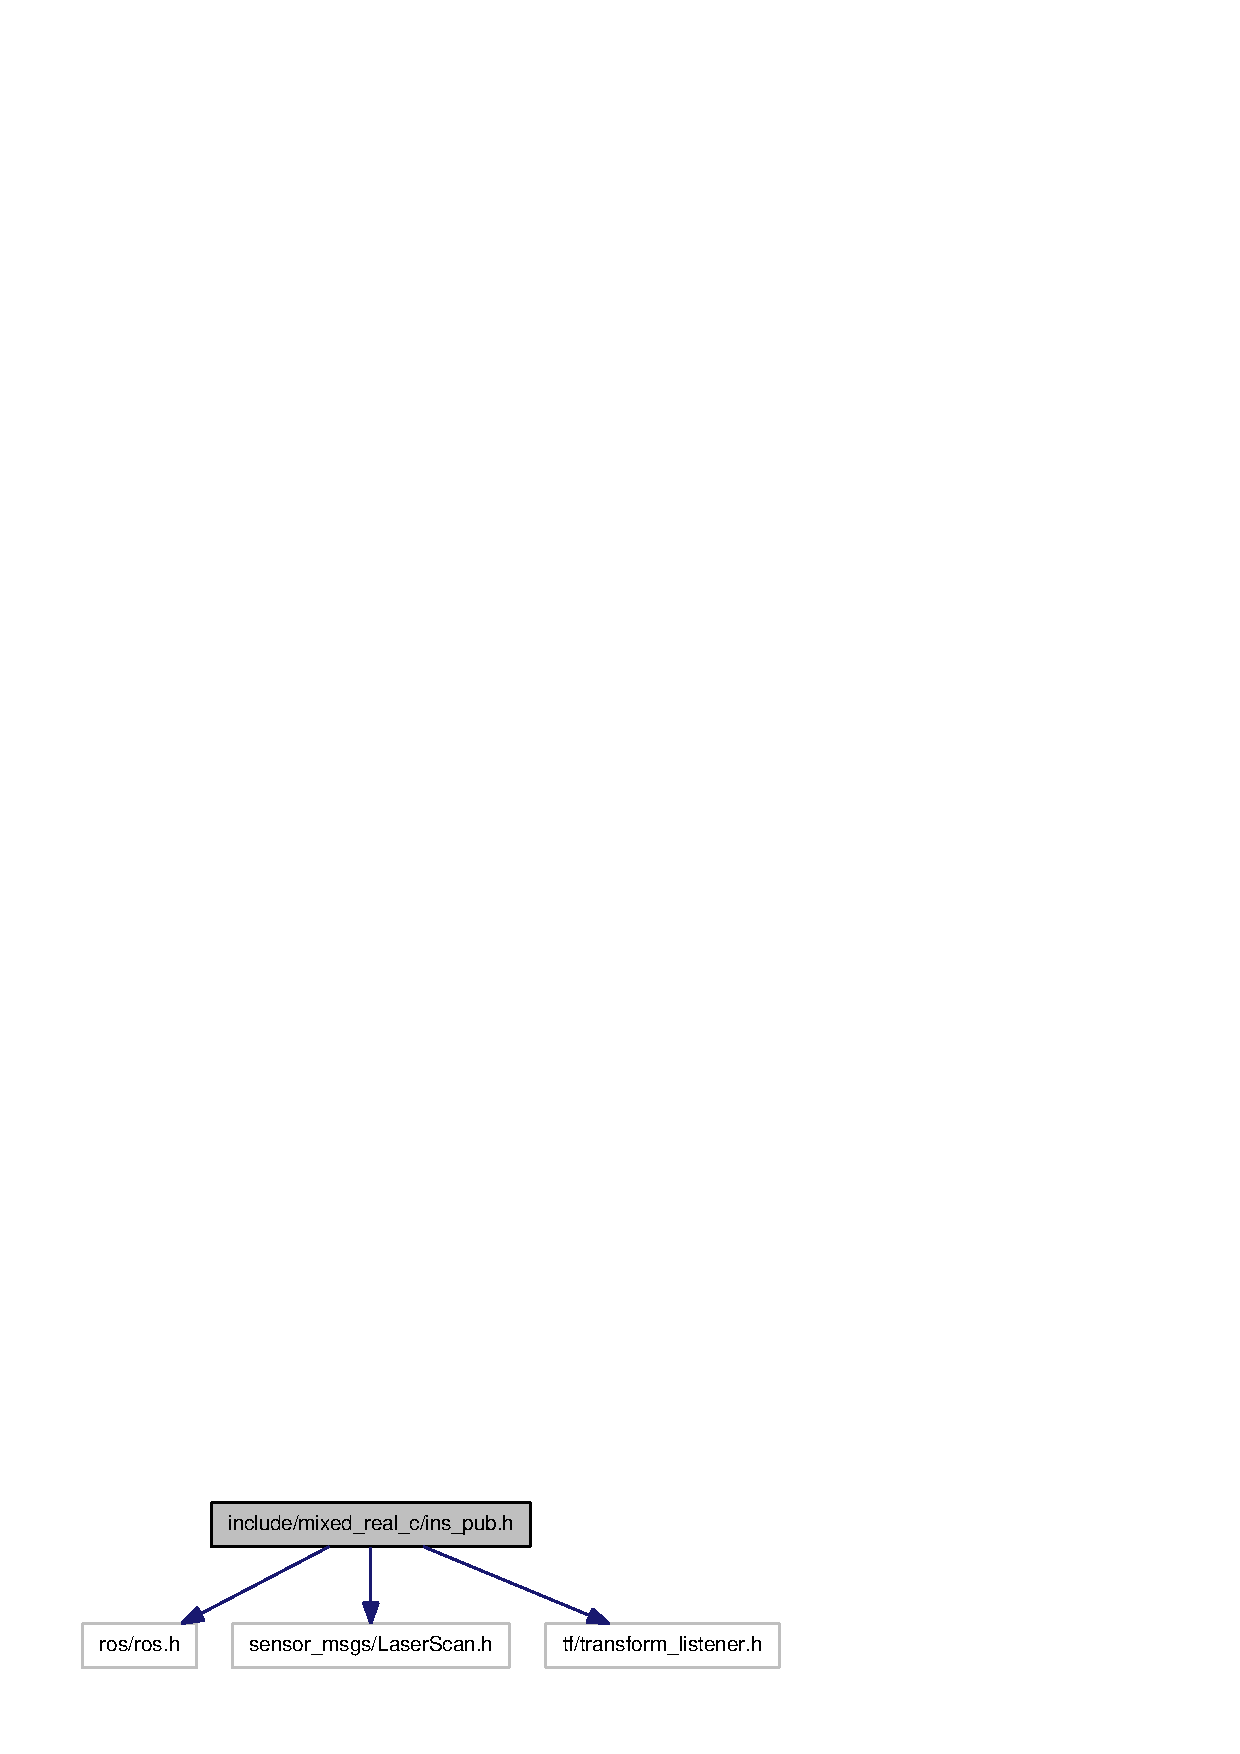
\includegraphics[width=378pt]{ins__pub_8h__incl}
\end{center}
\end{figure}
This graph shows which files directly or indirectly include this file:\nopagebreak
\begin{figure}[H]
\begin{center}
\leavevmode
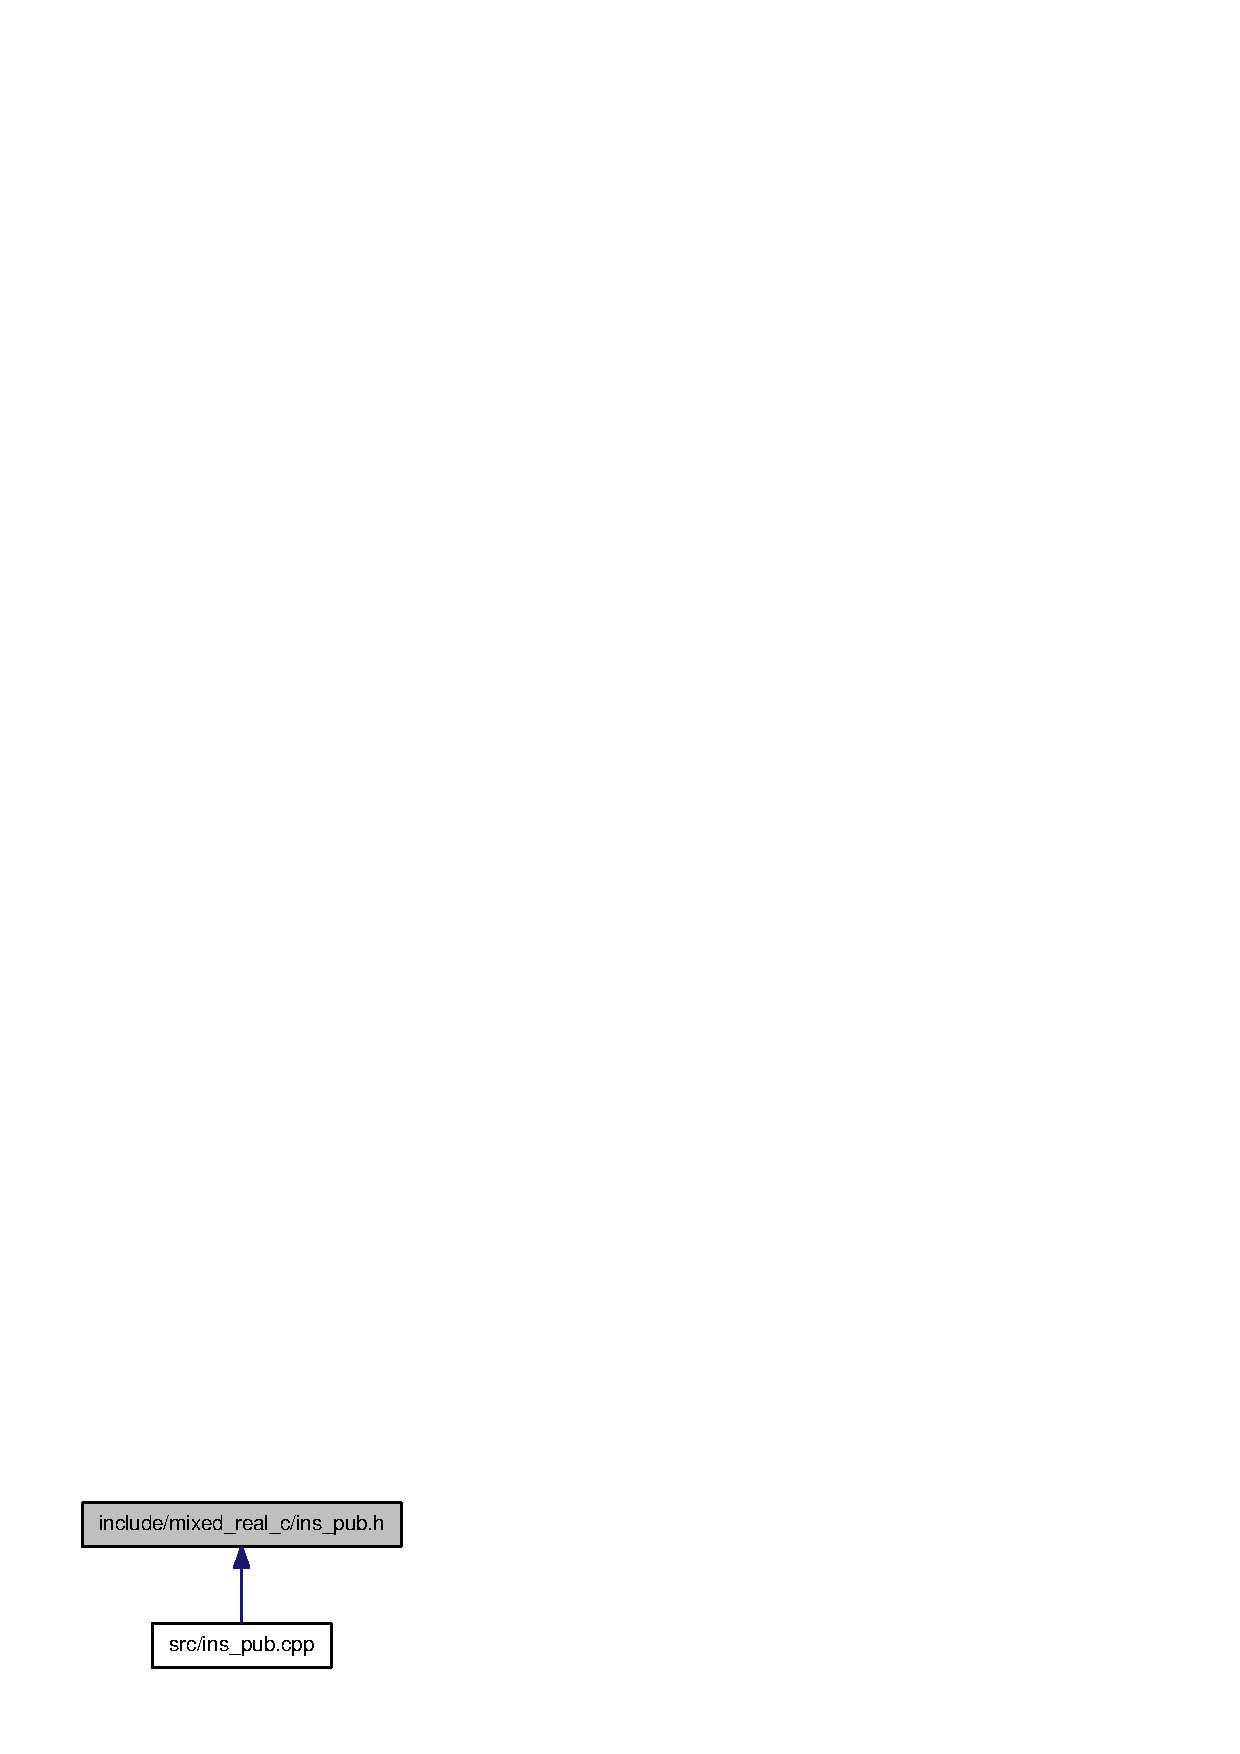
\includegraphics[width=196pt]{ins__pub_8h__dep__incl}
\end{center}
\end{figure}
\subsection*{Classes}
\begin{DoxyCompactItemize}
\item 
class {\bf insertObj}
\item 
struct {\bf preset}
\item 
class {\bf virtualObject}
\end{DoxyCompactItemize}
\subsection*{Defines}
\begin{DoxyCompactItemize}
\item 
\#define {\bf DIS\_\-STRENGTH}~0.008
\item 
\#define {\bf doNotCross}~1
\item 
\#define {\bf LEN\_\-FRONT\_\-VECT}~2
\item 
\#define {\bf PI}~3.14159265359
\end{DoxyCompactItemize}
\subsection*{Typedefs}
\begin{DoxyCompactItemize}
\item 
typedef struct {\bf preset} {\bf Preset}
\end{DoxyCompactItemize}
\subsection*{Variables}
\begin{DoxyCompactItemize}
\item 
double {\bf las\_\-ang\_\-max} = PI$\ast$0.75
\item 
double {\bf las\_\-ang\_\-min} = -\/PI$\ast$0.75
\item 
double {\bf MAX\_\-ANGLE} = 2$\ast$PI/0.75
\item 
sensor\_\-msgs::LaserScan {\bf mixed\_\-scan}
\item 
double {\bf noise} = DIS\_\-STRENGTH
\item 
{\bf insertObj} $\ast$ {\bf pIObj}
\item 
int {\bf test\_\-info} = 0
\item 
double {\bf UNIT\_\-BTW\_\-LAS} = (PI/360.0)
\end{DoxyCompactItemize}


\subsection{Detailed Description}
Hlavickovy subor aplikacie na vkladanie virtualnych objektov do dat robota. \begin{DoxyAuthor}{Author}
Jakub Fisla (xfisla00) 
\end{DoxyAuthor}


Definition in file {\bf ins\_\-pub.h}.



\subsection{Define Documentation}
\index{ins\_\-pub.h@{ins\_\-pub.h}!DIS\_\-STRENGTH@{DIS\_\-STRENGTH}}
\index{DIS\_\-STRENGTH@{DIS\_\-STRENGTH}!ins_pub.h@{ins\_\-pub.h}}
\subsubsection[{DIS\_\-STRENGTH}]{\setlength{\rightskip}{0pt plus 5cm}\#define DIS\_\-STRENGTH~0.008}\label{ins__pub_8h_abedab1b196d80411e1ed102f2a367ccd}


Definition at line 28 of file ins\_\-pub.h.

\index{ins\_\-pub.h@{ins\_\-pub.h}!doNotCross@{doNotCross}}
\index{doNotCross@{doNotCross}!ins_pub.h@{ins\_\-pub.h}}
\subsubsection[{doNotCross}]{\setlength{\rightskip}{0pt plus 5cm}\#define doNotCross~1}\label{ins__pub_8h_a1f597718bbb741b6773d45c36555b214}


Definition at line 24 of file ins\_\-pub.h.

\index{ins\_\-pub.h@{ins\_\-pub.h}!LEN\_\-FRONT\_\-VECT@{LEN\_\-FRONT\_\-VECT}}
\index{LEN\_\-FRONT\_\-VECT@{LEN\_\-FRONT\_\-VECT}!ins_pub.h@{ins\_\-pub.h}}
\subsubsection[{LEN\_\-FRONT\_\-VECT}]{\setlength{\rightskip}{0pt plus 5cm}\#define LEN\_\-FRONT\_\-VECT~2}\label{ins__pub_8h_afa7a11fe6808d6f2d83b138660cfe938}


Definition at line 26 of file ins\_\-pub.h.

\index{ins\_\-pub.h@{ins\_\-pub.h}!PI@{PI}}
\index{PI@{PI}!ins_pub.h@{ins\_\-pub.h}}
\subsubsection[{PI}]{\setlength{\rightskip}{0pt plus 5cm}\#define PI~3.14159265359}\label{ins__pub_8h_a598a3330b3c21701223ee0ca14316eca}


Definition at line 27 of file ins\_\-pub.h.



\subsection{Typedef Documentation}
\index{ins\_\-pub.h@{ins\_\-pub.h}!Preset@{Preset}}
\index{Preset@{Preset}!ins_pub.h@{ins\_\-pub.h}}
\subsubsection[{Preset}]{\setlength{\rightskip}{0pt plus 5cm}typedef struct {\bf preset} {\bf Preset}}\label{ins__pub_8h_aba266741f5e08c118d22f0da93fe9e4a}
Struktura obsahujuca data virtualneho objektu. Obsahuje meno (name), x suradnice, y suradnice, a intenzitu nasnimaneho signalu 

\subsection{Variable Documentation}
\index{ins\_\-pub.h@{ins\_\-pub.h}!las\_\-ang\_\-max@{las\_\-ang\_\-max}}
\index{las\_\-ang\_\-max@{las\_\-ang\_\-max}!ins_pub.h@{ins\_\-pub.h}}
\subsubsection[{las\_\-ang\_\-max}]{\setlength{\rightskip}{0pt plus 5cm}double {\bf las\_\-ang\_\-max} = PI$\ast$0.75}\label{ins__pub_8h_ab83311036cf2c6243184887da554a036}


Definition at line 32 of file ins\_\-pub.h.

\index{ins\_\-pub.h@{ins\_\-pub.h}!las\_\-ang\_\-min@{las\_\-ang\_\-min}}
\index{las\_\-ang\_\-min@{las\_\-ang\_\-min}!ins_pub.h@{ins\_\-pub.h}}
\subsubsection[{las\_\-ang\_\-min}]{\setlength{\rightskip}{0pt plus 5cm}double {\bf las\_\-ang\_\-min} = -\/PI$\ast$0.75}\label{ins__pub_8h_a160d940f8bd263498c1641fca83f2585}


Definition at line 33 of file ins\_\-pub.h.

\index{ins\_\-pub.h@{ins\_\-pub.h}!MAX\_\-ANGLE@{MAX\_\-ANGLE}}
\index{MAX\_\-ANGLE@{MAX\_\-ANGLE}!ins_pub.h@{ins\_\-pub.h}}
\subsubsection[{MAX\_\-ANGLE}]{\setlength{\rightskip}{0pt plus 5cm}double {\bf MAX\_\-ANGLE} = 2$\ast$PI/0.75}\label{ins__pub_8h_ac32ec987dfc5022ee8e26d4f2fd05732}


Definition at line 31 of file ins\_\-pub.h.

\index{ins\_\-pub.h@{ins\_\-pub.h}!mixed\_\-scan@{mixed\_\-scan}}
\index{mixed\_\-scan@{mixed\_\-scan}!ins_pub.h@{ins\_\-pub.h}}
\subsubsection[{mixed\_\-scan}]{\setlength{\rightskip}{0pt plus 5cm}sensor\_\-msgs::LaserScan {\bf mixed\_\-scan}}\label{ins__pub_8h_aad1de035bfed6f3c908d6f72a2ec2d1e}


Definition at line 87 of file ins\_\-pub.h.

\index{ins\_\-pub.h@{ins\_\-pub.h}!noise@{noise}}
\index{noise@{noise}!ins_pub.h@{ins\_\-pub.h}}
\subsubsection[{noise}]{\setlength{\rightskip}{0pt plus 5cm}double {\bf noise} = DIS\_\-STRENGTH}\label{ins__pub_8h_aedb3acb007b8cca8efc63eed08f45705}


Definition at line 88 of file ins\_\-pub.h.

\index{ins\_\-pub.h@{ins\_\-pub.h}!pIObj@{pIObj}}
\index{pIObj@{pIObj}!ins_pub.h@{ins\_\-pub.h}}
\subsubsection[{pIObj}]{\setlength{\rightskip}{0pt plus 5cm}{\bf insertObj}$\ast$ {\bf pIObj}}\label{ins__pub_8h_aba39bde455b1a2ce9784bec3b52ebd49}


Definition at line 86 of file ins\_\-pub.h.

\index{ins\_\-pub.h@{ins\_\-pub.h}!test\_\-info@{test\_\-info}}
\index{test\_\-info@{test\_\-info}!ins_pub.h@{ins\_\-pub.h}}
\subsubsection[{test\_\-info}]{\setlength{\rightskip}{0pt plus 5cm}int {\bf test\_\-info} = 0}\label{ins__pub_8h_aba44f1379e8e30d4041e9f6d07fc33e0}


Definition at line 89 of file ins\_\-pub.h.

\index{ins\_\-pub.h@{ins\_\-pub.h}!UNIT\_\-BTW\_\-LAS@{UNIT\_\-BTW\_\-LAS}}
\index{UNIT\_\-BTW\_\-LAS@{UNIT\_\-BTW\_\-LAS}!ins_pub.h@{ins\_\-pub.h}}
\subsubsection[{UNIT\_\-BTW\_\-LAS}]{\setlength{\rightskip}{0pt plus 5cm}double {\bf UNIT\_\-BTW\_\-LAS} = (PI/360.0)}\label{ins__pub_8h_aa4a18312d42e276842d0bcd85bd42532}


Definition at line 30 of file ins\_\-pub.h.


\section{mainpage.dox File Reference}
\label{mainpage_8dox}\index{mainpage.dox@{mainpage.dox}}

\section{src/ins\_\-pub.cpp File Reference}
\label{ins__pub_8cpp}\index{src/ins\_\-pub.cpp@{src/ins\_\-pub.cpp}}


Implementacia aplikacie vkladania virtualnych objektov do dat robota v ROS-\/e.  


{\ttfamily \#include \char`\"{}mixed\_\-real\_\-c/ins\_\-pub.h\char`\"{}}\par
Include dependency graph for ins\_\-pub.cpp:\nopagebreak
\begin{figure}[H]
\begin{center}
\leavevmode
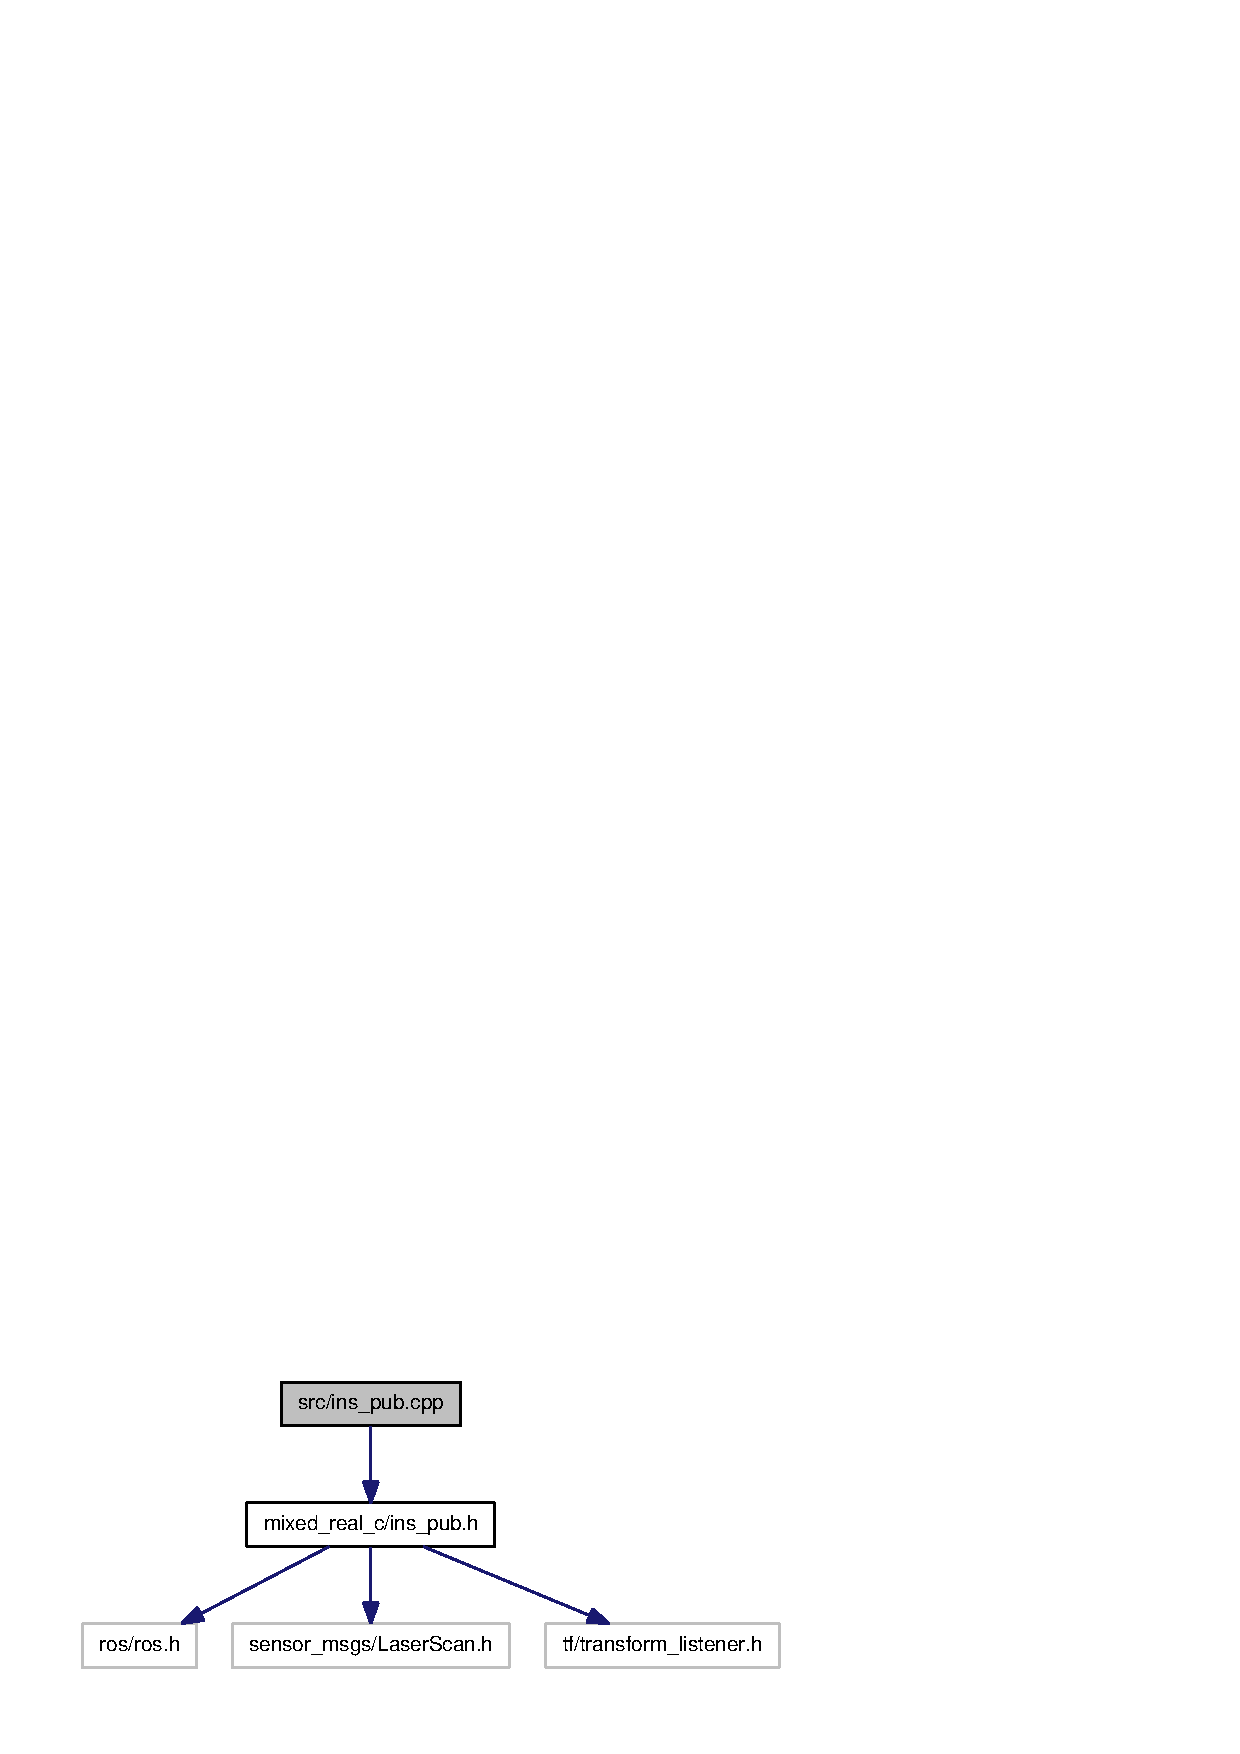
\includegraphics[width=378pt]{ins__pub_8cpp__incl}
\end{center}
\end{figure}
\subsection*{Functions}
\begin{DoxyCompactItemize}
\item 
bool {\bf isLeft} (tf::Vector3 a, tf::Vector3 b, tf::Vector3 c)
\item 
int {\bf main} (int argc, char $\ast$$\ast$argv)
\item 
void {\bf scanCallback} (const sensor\_\-msgs::LaserScan::ConstPtr \&scan)
\end{DoxyCompactItemize}


\subsection{Detailed Description}
Implementacia aplikacie vkladania virtualnych objektov do dat robota v ROS-\/e. \begin{DoxyAuthor}{Author}
Jakub Fisla (xfisla00) 
\end{DoxyAuthor}


Definition in file {\bf ins\_\-pub.cpp}.



\subsection{Function Documentation}
\index{ins\_\-pub.cpp@{ins\_\-pub.cpp}!isLeft@{isLeft}}
\index{isLeft@{isLeft}!ins_pub.cpp@{ins\_\-pub.cpp}}
\subsubsection[{isLeft}]{\setlength{\rightskip}{0pt plus 5cm}bool isLeft (
\begin{DoxyParamCaption}
\item[{tf::Vector3}]{a, }
\item[{tf::Vector3}]{b, }
\item[{tf::Vector3}]{c}
\end{DoxyParamCaption}
)}\label{ins__pub_8cpp_ac25751b0a6fa470844bfcce02c481fc4}
Funkcia urcuje polhu bodu c voci usecke $|$ab$|$


\begin{DoxyParams}{Parameters}
{\em a} & Vektor bodu a \\
\hline
{\em b} & Vektor bodu b \\
\hline
{\em c} & Vektor bodu c\\
\hline
\end{DoxyParams}
\begin{DoxyReturn}{Returns}
Vracia true ak je bod c vlavo od usecky $|$ab$|$, inac vracia false 
\end{DoxyReturn}


Definition at line 292 of file ins\_\-pub.cpp.

\index{ins\_\-pub.cpp@{ins\_\-pub.cpp}!main@{main}}
\index{main@{main}!ins_pub.cpp@{ins\_\-pub.cpp}}
\subsubsection[{main}]{\setlength{\rightskip}{0pt plus 5cm}int main (
\begin{DoxyParamCaption}
\item[{int}]{argc, }
\item[{char $\ast$$\ast$}]{argv}
\end{DoxyParamCaption}
)}\label{ins__pub_8cpp_a3c04138a5bfe5d72780bb7e82a18e627}
Hlavna funkcia programu, spusta vsetky ostatne funkcie

\begin{DoxyReturn}{Returns}
Vracai navratovu hodnotu programu 
\end{DoxyReturn}


Definition at line 530 of file ins\_\-pub.cpp.

\index{ins\_\-pub.cpp@{ins\_\-pub.cpp}!scanCallback@{scanCallback}}
\index{scanCallback@{scanCallback}!ins_pub.cpp@{ins\_\-pub.cpp}}
\subsubsection[{scanCallback}]{\setlength{\rightskip}{0pt plus 5cm}void scanCallback (
\begin{DoxyParamCaption}
\item[{const sensor\_\-msgs::LaserScan::ConstPtr \&}]{scan}
\end{DoxyParamCaption}
)}\label{ins__pub_8cpp_abe3232211edb2291f70f7fee36aefe12}
Funkcia v ktorej je spristupnena odoberana sprava z topiku


\begin{DoxyParams}{Parameters}
{\em scan} & Ukazovatel na prijatu spravu \\
\hline
\end{DoxyParams}


Definition at line 499 of file ins\_\-pub.cpp.


\printindex
\end{document}
